\documentclass[a4paper]{article}
\usepackage[margin=0mm]{geometry}
\usepackage{tikz}
\pagestyle{empty}

\begin{document}
\thispagestyle{empty}

\begin{tikzpicture}[remember picture,overlay]
  % Point de départ : coin haut-gauche de la page
  % Puis on va à droite de 0.5cm et on descend de 0.5cm
  \begin{scope}[shift={(current page.north west)}, xshift=0.5cm, yshift=-0.5cm]

    % Grille 19 x 28 (pas de 1 cm)
    \draw[step=1cm, line width=0.2pt] (0,0) grid (19cm,-27cm);

    % Surligne (bord épais) les cases "noires" du damier
    \foreach \i in {0,...,18} { % 19 colonnes -> 0..18
        \foreach \j in {0,...,27} { % 28 lignes -> 0..27

            % Test si i est impair
            \pgfmathtruncatemacro{\icol}{mod(\i+1,2)}

            % Test damier
            \pgfmathtruncatemacro{\parity}{mod(\i+\j,2)}

            \ifnum\icol=1          % seulement colonnes impaires
                \ifnum\parity=0    % motif damier
                    \draw[line width=1.0pt] (\i cm,-\j cm) rectangle ++(1cm,-1cm);
                \fi
            \fi
        }
    }
  \end{scope}
\end{tikzpicture}

\end{document}
